\documentclass[12pt]{article}
  \usepackage[francais]{babel}
  \AddThinSpaceBeforeFootnotes % à insérer si on utilise \usepackage[french]{babel}
  \FrenchFootnotes % à insérer si on utilise \usepackage[french]{babel}
  \usepackage[T1]{fontenc}
  \usepackage[utf8]{inputenc}
  \usepackage{graphicx}
  \usepackage[left=2.5cm,right=2.5cm,top=2.5cm,bottom=2.5cm]{geometry}
  \usepackage{array}
  \usepackage{booktabs}
  \usepackage[squaren,Gray]{SIunits}  % Unité ex: $\unit{5 \cdot 10^{-6}}{\meter}$
  \usepackage{colortbl}               % Pour les couleur des cellules (tableau)
  \usepackage{amsmath}				  % Pour les formules mathématiques
  \usepackage{upgreek}                % Pour les lettres greque
  %\usepackage{fullpage}	          % plus petites marges
  \usepackage{verbatim}				  % Pour de long commentaires
  \usepackage[lofdepth,lotdepth]{subfig}       % Faire des sous-figures
  \usepackage{url}
  \usepackage{colortbl}               % pour les couleur des cellules (tableau)
  \usepackage{indentfirst}
  \usepackage{multirow}
  \usepackage{xfrac}
  \usepackage{wrapfig}
  \usepackage{enumitem}               % Liste personnalisée
  \frenchbsetup{StandardLists=true}   % Empêche conflits entre enumitem et babel
  \usepackage{placeins}   % place une barrière pour que l'image/table soit derrière \FloatBarrier
  \usepackage{lastpage} 
  \usepackage{titling}
  \usepackage{lmodern}
  \usepackage{booktabs}
  \usepackage{etoolbox}
  \usepackage[most]{tcolorbox}
  
  
  %Change la taille de police
  \newcommand\ChangeRT[1]{\noalign{\hrule height #1}}
  
\graphicspath{{images/}}

  
  %Création  d'une nouvelle commande pour faire référence à une Figure
  %Exemple : \appelFigure{schema} donne : Figure 1 (en italique)
  \newcommand{\appelFigure}[1]{
    \textit{Figure \ref{#1}}
  }
      
  %%Création commande pour insérer image avec nom de figure directement
  %\newcommand{nomDeTaCommande}[nombreArguments]{CodeLaTeX}
  %\insertImage[position]{image_path}{scale}{Titre_figure}{label}
  \newcommand{\insertImage}[5][center]{
      \begin{#1}
      \includegraphics[scale=#3]{#2}
      \captionof{figure}{#4} 
      \label{#5}
      \end{#1}
  }

  % Affichage des frames pour commande cisco
  \newtcblisting{cisco}[1][]{size=fbox, listing only, listing options={style=tcblatex,basicstyle=\ttfamily\scriptsize,tabsize=2,language=sh},title=#1}

  %En-tête et pied de page personalisé
  \usepackage{fancyhdr}
  \pagestyle{fancy}
  \fancyhf{}
  \setlength\parindent{0pt} %Supprime les alinéa
  \setlength{\parskip}{8pt} %Augmente l'espace entre paragraphe
  %Bottom numbering page
  \renewcommand{\headrulewidth}{1pt}
  \fancyhead[L]{
\includegraphics[scale=.2]{heia-fr-logo.png}}
  \fancyhead[R]{\theauthor}
  
  \renewcommand{\footrulewidth}{1pt}
  \fancyfoot[R]{\textbf{Page \thepage\ sur \pageref{LastPage}}} 
%  \fancyfoot[L]{\leftmark}

  \setlength\parindent{0pt} %Supprime les alinéa
  \setlength{\parskip}{8pt} %Augmente l'espace entre paragraphe


\title{MATLAB  } 
\author{\textsl{Marc} \textsc{Roten}}
\date{}

\begin{document}
    \begin{titlepage}
        \begin{center}
            
\includegraphics[scale=.4]{Img/heia-fr-logo.png}\\[1.3cm]
            
            \rule{\linewidth}{0.3mm} \\[0.3cm]
            {\huge \bfseries Signaux système\\[0.5cm]} 
           % {\Large Effet photoélectrique}\\[0.2cm]
            {\Large  Labo 01 Matlab }
            \rule{\linewidth}{0.3mm} \\[0.8cm]
            \noindent
            \begin{minipage}[t]{0.4\textwidth}
                \begin{flushleft} \large
                    \emph{Auteur :}\\
                    \theauthor
                \end{flushleft}
            \end{minipage}
            \begin{minipage}[t]{0.4\textwidth} 
                \begin{flushright} \large
                    \emph{Professeur:}\\
                    \textsl{Daniel} \textsc{ Oberson}\\ 
                \end{flushright} 
                \vfill
            \end{minipage}\\[1.3cm]
            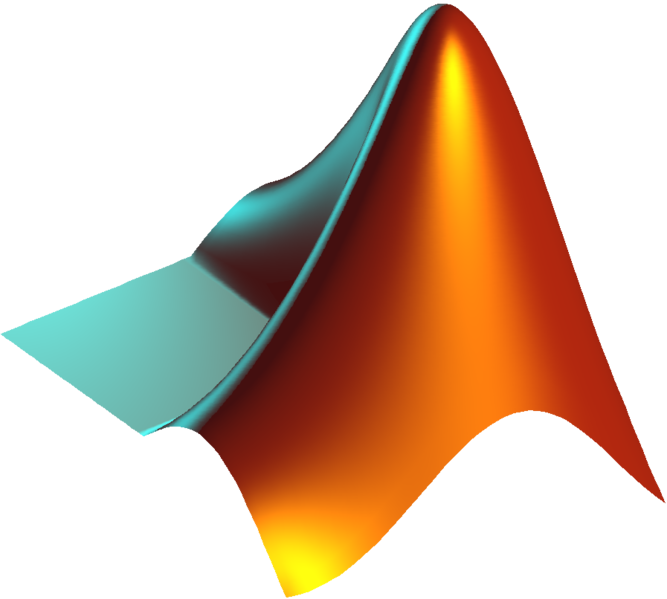
\includegraphics[scale=0.5]{Img/title.jpg}\\[1.5cm]
            \vspace*{1\baselineskip}
            \today \\[0.7cm]
        \end{center}
    \end{titlepage}
    \tableofcontents
    \clearpage
% \insertImage{Img/photo.PNG}{0.8}{Schéma explicatif}{}

% \section{voici comment faire un chapitre}

%     \subsection{Voici comment faire un sous chapitre}

% \section{des commandes}
%     \subsection{commande cisco}
    
%     \begin{cisco}[une commande sympa type cisco]
%       un texte lambda
%     \end{cisco}
    
%     \subsection{commande cisco allégée}
    
%     \begin{cisco}
%       un texte lambda
%     \end{cisco}
    
    
%     \subsection{commande pour mettre une image}
    
%     \insertImage{Img/1.PNG}{echelle pour l'image source = 1}{texte dessous l'image}{référence vers l'objet}
%     \insertImage{Img/1.JPG}{0.6}{voici une image}{myImg}
%	  \ref{myImg}
\section{Introduction}
Ce travail personnel individuel a pour objectif de nous permettre de prendre en main l'outil Matlab. On va procéder à  la construction et à l'affichage de signaux élémentaires via l'outil Matlab. On va aussi procéder à l'analyse fréquentielle de différents signaux.

\section{Travail à réaliser}
\subsection{Signal d'entrée point à point}

\insertImage{Img/donnee1.JPG}{0.75}{Donnée}{donnée1}

\insertImage{Img/q1.png}{0.75}{Résultat obtenu}{q1}






\subsection{Générer des séries}
Faites une nouvelle section dans votre script Matlab avec %% et générez les signaux suivant:

$$ X_{1}(t)=sin(2\pi f t)+\frac{1}{3}sin(2\pi 3ft)+\frac{1}{5}sin(2\pi 5ft)+\frac{1}{7}sin(2\pi 7ft)...$$

$$ X_{2}(t)=cos(2\pi ft)+\frac{1}{3^2}cos(2\pi 3ft)+\frac{1}{5^2}cos(2\pi 5ft)+\frac{1}{7^2}cos(2\pi 7ft)...$$

$$f = 2Hz~et -1[s]<t<1[s]$$

Affichez les deux signaux sur le même graphique. Quels signaux obtient-on lorsque l'on augmente le nombre de termes des sommes?

\insertImage{Img/q2.png}{0.75}{Résultat obtenu}{q2}

On voit en Figure \ref{q2} que le signal $X_1(t)$ est un signal carré, et que le signal $X_2(t)$est un signal triangle. Lorsque l'on augmente le nombre de termes à notre équation, le graphique devient de plus en plus précis, et même crée un signal carré si on tend vers l'infini. Mais ça, on le génèrera au point optionnel 3.1.

\newpage
\subsection{Représentation fréquentielle}

En vous appuyant sur la documentation en annexe, calculez dans Matlab la FFT des signaux $x_1 (t) et x_2 (t)$ avec la fondamentale et 3 harmoniques sans fenêtre de pondération et affichez le résultat graphiquement.

Déterminez depuis le résultat des calculs des FFT, les amplitudes et les phases des composantes fréquentielles $x_1 (t) et x_2 (t)$.

\subsection{Analyse fréquentielle}
Utilisez alors la fonction sound() de Matlab pour écouter la note de piano et la note de guitare enregistrées. Puis, en faisant une analyse fréquentielle par la FFT comme précédemment, déterminez la fréquence des notes enregistrées dans ces deux fichiers. 

Il faut utiliser la fonction $load <filename>$

Ces notes sont-elles différentes? Le son entendu est-il différent? Qu'en concluez-vous?





\newpage
\section{Travail optionnel}
en faire au moins un
\subsection{Fonction génération automatique de signal}
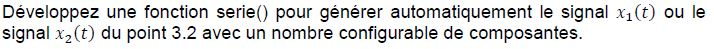
\includegraphics[scale=.8]{Img/o1.JPG}


\subsection{Recrée le signal avec ses 3 fondamentales}
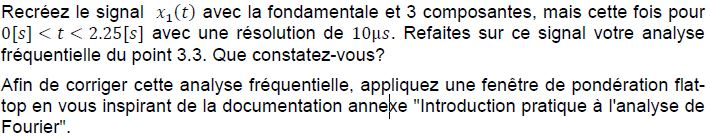
\includegraphics[scale=.8]{Img/o2.JPG}

\subsection{Manipulation FFT piano et/ou guitare}
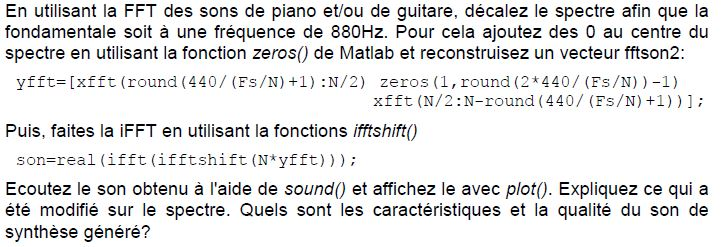
\includegraphics[scale=.8]{Img/o3.JPG}

\section{Conclusion}
Par ce travail j'ai pu m'entraîner sur l'outil Matlab. Apprendre de nouvelles fonctions de génération de fréquence. 

L'analyse fréquentielle et les séries sont un bon rappel des connaissances acquises durant l'apprentissage durant la maturité et des connaissances acquises durant la première année.





\end{document}